\renewcommand\refname{Literaturverzeichnis}
\addcontentsline{toc}{section}{Literaturverzeichnis}
\printbibliography
\cleardoublepage
\listoffigures


\clearpage

\appendix

\section{Aufgabenstellung}
\begin{figure}[h]
    \centering
    \begin{minipage}[b]{0.8\textwidth}
        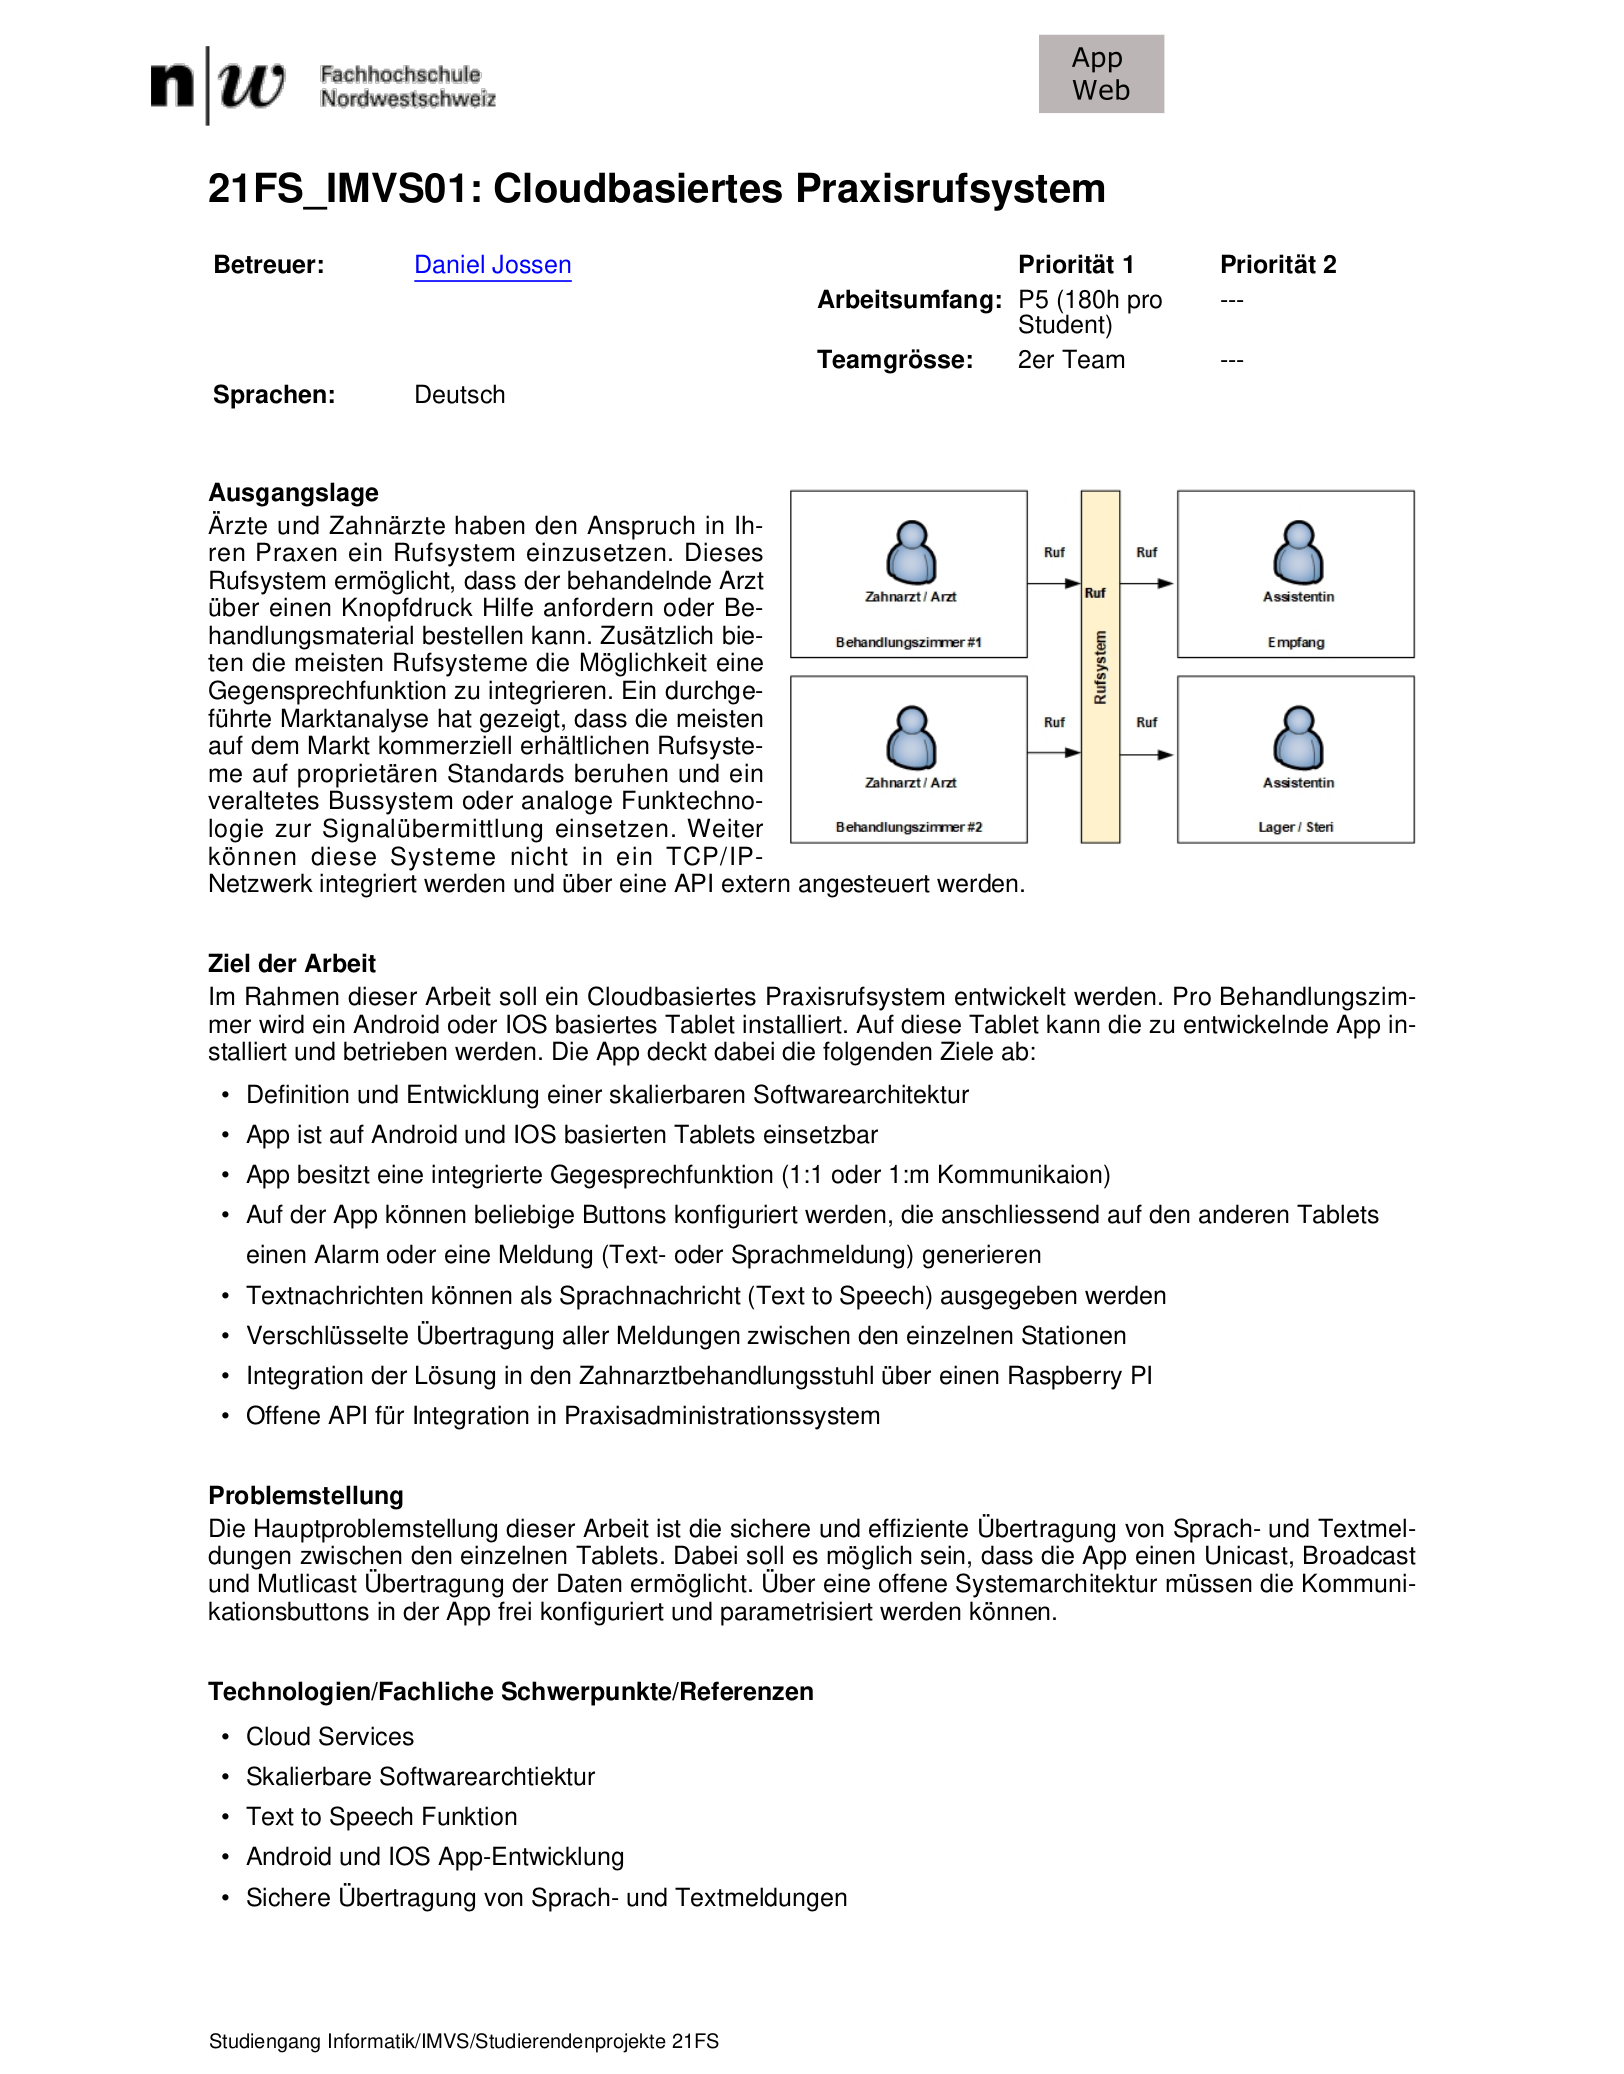
\includegraphics[width=\textwidth]{graphics/aufgabenstellung}
        \caption{Aufgabenstellung}
    \end{minipage}
\end{figure}

\clearpage


\section{Quellcodeverwaltung}

Sämtlicher Quellcode der im Rahmen des Projektes entsteht, wurde mit Git verwaltet. Der Quellcode ist für Berechtigte unter dem Projekt IP5-Cloudbasiertes-Praxisrufsystem auf github.com einsehbar.
(Referenz https://github.com/IP5-Cloudbasiertes-Praxisrufsystem). Berechtigungen können bei Joshua Villing oder Kevin Zellweger angefordert werden.

\section{Benutzerhandbuch}

\subsubsection*{Mobile Client}

\textbf{Anmeldung und Konfiguration}

\begin{enumerate}
    \item Mobile Client Applikation öffnen
    \item Anmeldedaten eingeben und bestätigen
    \item Gewünschte Konfiguration auswählen
\end{enumerate}

\textbf{Benachrichtigung empfangen}

\begin{enumerate}
    \item In Mobile Client anmelden.
    \item In Navigationsleiste (unten) "Home" auswählen.
    \item Button mit dem gewünschten Titel antippen.
    \item Die Benachrichtigung wird automatisch versendet.
\end{enumerate}

\textbf{Benachrichtigung Auflisten und Quittieren}

\begin{enumerate}
    \item In Mobile Client anmelden.
    \item In Navigationsleiste (unten) "Inbox" auswählen.
    \item In dieser Ansicht sehen Sie alle empfangenen noch nicht quittierten Benachrichtigungen.
    \item Zum Quittieren einer Benachrichtigung kann diese angetippt werden.
\end{enumerate}

\textbf{Abmeldung}

\begin{enumerate}
    \item Mobile Client Applikation öffnen
    \item Auf den Namen in der Kopfleiste tippen
    \item Logout bestätigen
\end{enumerate}

\subsubsection*{Admin UI}

\textbf{Anmeldung}

\begin{enumerate}
    \item Admin UI im Browser öffnen
    \item Anmeldedaten eingeben und bestätigen. Die Anmeldedaten erhalten Sie nach Installation des Systems vom Betreiber.
\end{enumerate}

\textbf{Einträge hinzufügen}
\begin{enumerate}
    \item Melden Sie sich im Admin UI an.
    \item Wählen Sie auf der Linken Seite die Kategorie die Sie verwalten möchten.
    \item Auf dieser Seite können Sie nun Einträge zur gewählten Kategorie verwalten:
    \begin{itemize}
        \item Klicken Sie oben rechts auf die Schaltfläche "Create" um einen neuen Eintrag zu erstellen.
        \item Klicken Sie auf einen Eintrag in der Liste um ihn zu bearbeiten.
        \item Klicken Sie die Checkbox auf der Linken Seite eines Eintrages und dann auf die Schaltfläche "löschen" um einen Eintrag zu löschen.
    \end{itemize}
\end{enumerate}

\textbf{Praxisruf konfigurieren}
\begin{enumerate}
    \item Melden Sie sich im Admin UI an.
    \item Erfassen Sie in der Kategorie "User" pro Praxiszimmer einen Benutzer.
    \item Erfassen Sie in der Kategorie "Client" pro Gerät und Zimmer einen Eintrag und weisen Sie ihn dem Benutzer des entsprechenden Zimmers zu.
    \item Erfassen Sie in der Kategorie "Notification Types" alle Benachrichtigungen die Sie zur Verfügung stellen möchten.
    \item Erfassen Sie in der Kategorie "Configurations" pro Gerät und Zimmer einen Eintrag und weisen es dem entsprechenden Client zu.
    \item Unter Notification Types können die Benachrichtigungen auswählen, die auf diesem Gerät zum Versenden verfügbar sind.
    \item Unter Rule Parameters können Sie Regeln definieren, welche Benachrichtigungen diesem Client zugestellt werden.
\end{enumerate}

\clearpage


\section{Installationsanleitung}

\subsubsection*{Mobile Client}
\textbf{TODO} \\
?? Cloud Service url configuration \\
?? FCM Integration configuration \\

\subsubsection*{Admin UI}

Im Folgenden wird beschrieben wie die Admin UI Applikation mit AWS betrieben werden kann.

\begin{enumerate}
    \item AWS Amplify Service aufsetzen:
    \begin{enumerate}
        \item Amazon Webservice unterstützt die Anbdingun von Github, Gitlab, BitBucket und AWS CodeCommit. Stellen Sie sicher, dass der Quellcode der Admin UI Applikation in einem Git Repository zur Verfügung steht.
        \item Folgen Sie den Schritten in der \href{https://docs.aws.amazon.com/amplify/latest/userguide/getting-started.html}{\textit{offiziellen Anleitung}}.\cite{aws-amplify}
    \end{enumerate}
    \item Verbindung zum Cloud Service konfigurieren:
    \begin{enumerate}
        \item Öffnen sie die AWS Amplify Konsole für die in Schritt 1 erstellte Applikation.
        \item Wählen Sie den Menüpunkt "Environment Variables"
        \item Erstellen Sie eine neue Variable mit dem Namen REACT\_APP\_BACKEND\_BASE\_URI. Setzten Sie als Wert dafür die Domain, unter welcher der Cloud Service erreichbar ist.
    \end{enumerate}
    \item Konfigurieren Sie eine Domain für die Admin UI Applikation.
    \begin{enumerate}
        \item Folgen Sie dazu den Schritten in der \href{https://docs.aws.amazon.com/amplify/latest/userguide/custom-domains.html}{\textit{offiziellen Anleitung}}.\cite{aws-amplify-domain} folgen.
    \end{enumerate}
\end{enumerate}

\subsubsection*{Cloud Service}

Im Folgenden wird beschrieben wie die Cloud Service Applikation mit AWS betrieben werden kann.

\begin{enumerate}
    \item Stellen Sie sicher, dass der Quellcode der Cloud Service Applikation in einem Git Repository bei einem der Anbieter Github, Gitlab, BitBucket oder AWS CodeCommit zur Verfügung steht.
    \item Erstellen Sie einen mit AWS ein Elastic Beanstalk Environment.
    \begin{enumerate}
        \item Folgen Sie dazu der \href{https://docs.aws.amazon.com/elasticbeanstalk/latest/dg/GettingStarted.CreateApp.html}{\textit{offiziellen Anleitung}}\cite{aws-elastic}
        \item Wählen Sie unter Plattform "Java" und die dazugehörigen Standardeinstellungen.
        \item Wählen Sie unter Application Code "Sample Application".
    \end{enumerate}
    \item Erstellen sie mit AWS RDS eine Datenbank für die Cloud Service Applikation
    \begin{enumerate}
        \item In Beanstalk Console
        \item Folgen Sie der \href{https://docs.aws.amazon.com/elasticbeanstalk/latest/dg/using-features.managing.db.html}{\textit{offiziellen Anleitung}}\cite{aws-elastic-rds} um eine Relationale Datenbank an das Beanstalk Environment anzubinden.
        \item Wählen Sie als Datenbank Engine "postgres" in der Version 13.3.
        \item Wenn sie oben genannter Anleitung folgen, ist keine weitere Konfiguration für die Datenbankanbindung im Cloud Service nötig.
        Sollten Sie wählen, die Datenbank auf eine andere Art zu Betreiben müssen in Schritt 4 die Umgebungsvariablen RDS\_HOSTNAME, RDS\_PORT, RDS\_DB\_NAME, RDS\_USERNAME und RDS\_PASSWORD mit den entsprechenden Werten konfiguriert werden.
    \end{enumerate}
    \item Definieren Sie die nötigen Umgebungsvariablen für die Cloud Service Applikation:
    \begin{enumerate}
        \item Folgen Sie der \href{https://docs.aws.amazon.com/elasticbeanstalk/latest/dg/environments-cfg-softwaresettings.html}{\textit{offiziellen Anleitung}}\cite{aws-elastic-env} um die nötigen Umgebungsvariablen zu setzen:
        \item Name: FCM\_CREDENTIALS, Wert: Firebase Credentials mit Base 64 Encoded\footnote{Siehe Installationsanleitung Firebase Messaging}
        \item Name: SPRING\_PROFILES\_ACTIVE, Wert: aws.
    \end{enumerate}
    \item Konfigurieren Sie AWS CodeBuild um die Cloud Service Applikation mit AWS bauen zu können.
    \begin{enumerate}
        \item Öffnen Sie die AWS Console und wählen Sie unter Services "Code Pipeline" aus.
        \item Wählen Sie die Option "Create build project".
        \item Geben Sie unter Project Configuration einen passenden Namen ein.
        \item Wählen Sie unter Source den gewünschten Anbieter und geben Sie die Repository URl sowie die gewünschte Version (Branch Name) ein.
        \item Wählen Sie unter Buildspec "Use a buildspec file". Die projektspezifische Build Konfiguration ist in der Cloud Service Applikation bereits enthalten.
        \item Bestätigen Sie die Eingaben.
    \end{enumerate}
    \item Konfigurieren Sie AWS CodePipeline um die Cloud Service Applikation zu installieren:
    \begin{enumerate}
        \item Öffnen Sie die AWS Console und wählen Sie unter Services "Code Pipeline" aus.
        \item Wählen Sie die Option "Create New Pipeline".
        \item Geben Sie in Schritt 1 einen Namen für die Pipeline an und wählen Sie "Next".
        \item Wählen Sie in Schritt 2 gewünschten Anbieter und folgen sie dem Wizard um das Git Repository des Cloud Services anzubinden.
        \item Wählen Sie in Schritt 3 AWS CodeBuild und das CodeBuild Projekt welches Sie in Schritt 3 erstellt haben.
        \item Wählen Sie in Schritt 4 AWS Elastic Beanstalk und die in Schritt 2 definierten Instanzen.
        \item Bestätigen Sie die Eingabem.
    \end{enumerate}
    \item Stellen Sie sicher, dass die installierete Cloud Service Applikation über HTTPS erreichbar ist. Dies ist für die Kommunication mit Mobile Client Instanzen zwingend notwendig.
    \begin{enumerate}
        \item Folgen Sie dazu der offiziellen Anleitung\href{https://aws.amazon.com/premiumsupport/knowledge-center/elastic-beanstalk-https-configuration/}{\textit{offiziellen Anleitung}}\cite{aws-elastic-https}.
        \item Am Cloud Service sind dabei keine Änderungen nötig. 
    \end{enumerate}
    \item Erstellen Sie einen Adminstrator Account für das Admin UI.
    \begin{enumerate}
        \item Richten Sie den Datenbankzugriff auf die in Schritt 3 erstellte Datenbank gemäss der \href{https://docs.aws.amazon.com/AmazonRDS/latest/UserGuide/USER_ConnectToPostgreSQLInstance.html}{\textit{offiziellen Anleitung}}\cite{aws-elastic-rds-access}. ein.
        \item Passen Sie die Parameter in folgenden Script an und führen es auf der Datenbank aus:
        \lstinputlisting[caption=createadmin.sql,language=sql,label={lst:CreateAdmin.java}]{listings/createadmin.sql}

    \end{enumerate}

\end{enumerate}


\clearpage


\clearpage

\section{Features und Testszenarien}

\subsubsection*{F01 - Benachrichtigungen Versenden}
\begin{tabbing}
    Left \= Middle \= Right \= Right \kill
    Scenario S01: \> \> \> Benachrichtigung versenden\\ \\
    Given:  \> \> \> Benutzer ist vollständig angemeldet\\
    And: \>    \> \> Mindestens ein Empfänger ist konfiguriert\\
    When:   \> \> \> Praxismitarbeiter tippt auf einen Benachrichtigungs-Button\\
    Then:   \> \> \> Benachrichtigung wird an den zentralen Cloud Service gesendet\\
    And: \>    \> \> Benachrichtigung wird an alle Mobile Clients versendet\\
    \> \>  \> die sich für diese Benachrichtigung subscribed haben weitergeleitet\\
    And:   \> \> \> Praxismitarbeiter erhält optische Rückmeldung, dass Benachrichtigung versendet wurde\\

    \\
    Scenario S02: \>  \> \> Keine Empfänger konfiguriert\\ \\
    Given:  \> \> \> Benutzer ist vollständig angemeldet\\
    And:  \> \>   \> Kein Empfänger ist konfiguriert\\
    When:  \> \>  \> Praxismitarbeiter tippt auf einen Benachrichtigungs-Button\\
    Then:  \> \>  \> Benachrichtigung wird an den zentralen Cloud Service gesendet\\
    And:  \> \>   \> Benachrichtigung wird nicht weitergeleitet\\

\end{tabbing}


\subsubsection*{F02 - Benachrichtigungen Empfangen}
\begin{tabbing}
    Left \= Middle \= Right \= Right  \kill

    Scenario S03: \>  \> \> Empfangen\\ \\
    Given: \>  \> \>  Eine Benachrichtigung wurde von Mobile Client versendet\\
    When: \>  \> \>   Cloud Service Notification an Empfänger Mobile Client weiterleitet\\
    Then: \>  \> \>   Wird die Benachrichtigung vom Empfänger Mobile Client empfangen\\
    And: \>  \> \>    In einer Übersicht für empfangene Benachrichtigung angezeigt.\\

\end{tabbing}

\clearpage
\subsubsection*{F03 - Fehlgeschlagene Benachrichtigungen}

\begin{tabbing}
    Left \= Middle \= Right \= Right  \kill
    Scenario S04: \> \> \>  Fehler Rückmeldung\\ \\
    Given: \> \> \>   Eine Benachrichtigung wurde von Mobile Client versendet\\
    When: \> \> \>    Weiterleitung von Cloud Service Notification an Empfänger schlägt auf Service Seite fehl\\
    Then: \> \> \>    Der Praxismitarbeiter wird über den Fehler informiert\\
    And: \> \> \>     Der Praxismitarbeiter hat die Möglichkeit die fehlgeschlagenen Benachrichtigungen zu wiederholen\\
    \\
    Scenario S05: \> \> \>  Confirm Retry\\ \\
    Given: \> \> \>   Benachrichtigung ist fehlgeschlagen\\
    And: \> \> \>     Dialog zum Wiederholen wird angezeigt\\
    When: \> \> \>    Praxismitarbeiter bestätigt, dass wiederholt werden soll\\
    Then: \> \> \>    Der Cloudservice versucht erneut, die fehlgeschlagenen zuzustellen\\
    \\
    Scenario S06: \> \> \>  Cancel Retry\\ \\
    Given: \> \> \>   Benachrichtigung ist fehlgeschlagen\\
    And: \> \> \>     Dialog zum Wiederholen wird angezeigt\\
    When: \> \> \>    Praxismitarbeiter klick, dass nicht wiederholt werden soll\\
    Then: \> \> \>    Werden die fehlgeschlagenen nicht wiederholt\\
    And: \> \> \>     Zurück zur Notificationsansicht\\

\end{tabbing}

\subsubsection*{F04 - Über Benachrichtigungen Notifizieren}
\begin{tabbing}
    Left \= Middle \= Right \= Right  \kill
    Scenario S07: \> \> \>  Foreground\\ \\
    Given: \> \> \>   Mobile Client ist geöffnet\\
    When: \> \> \>    Eine Benachrichtigung wird vom Mobile Client empfangen\\
    Then: \> \> \>    Ein Audio Signal erklingt\\
    \\
    Scenario S08: \> \> \>  Background\\ \\
    Given: \> \> \>   Mobile Client läuft im Hintergrund\\
    When: \> \> \>    Eine Benachrichtigung wird vom Mobile Client empfangen\\
    Then: \> \> \>    Ein Audio Signal erklingt\\
    And: \> \> \>     Eine Push-Benachrichtigung wird angezeigt\\
    \\
    Scenario S09: \> \> \>  Nicht Quittiert\\ \\
    Given: \> \> \>   Mobile Client ist geöffnet\\
    And: \> \> \>     Eine Benachrichtigung wurde empfangen\\
    When: \> \> \>    Benachrichtigung wird nicht quittiert\\
    Then: \> \> \>    Ein Audio Signal erklingt\\
    And: \> \> \>     Das Audio Signal wiederholt sich alle 30 Sekunden, bis die Benachrichtigung quittiert wurde.\\
\end{tabbing}

\clearpage

\subsubsection*{F05 - Login Mobile Client}
\begin{tabbing}
    Left \= Middle \= Right \= Right  \kill
    Scenario S10: \> \> \>  Startbildschirm, wenn nicht angemeldet\\ \\
    Given: \> \> \>   Mobile Client is geöffnet\\
    When: \> \> \>  Benutzer ist nicht angemeldet\\
    Then: \> \> \>  Benutzer wird zum Login aufgefordert\\
    \\
    Scenario S11: \> \> \>  Startbildschirm, wenn angemeldet\\ \\
    Given: \> \> \>   Mobile Client is geöffnet\\
    When: \> \> \>  Benutzer ist angemeldet\\
    Then: \> \> \>  Konfiguration, die der Benutzer zuletzt gewählt hat, wird angezeigt\\
    And: \> \> \>    Benachrichtigungs-Buttons gemäss Konfiguration werden angezeigt.\\
    \\
    Scenario S12: \> \> \>  Anmelden korrekt\\ \\
    Given: \> \> \>  Benutzer ist nicht angemeldet\\
    And: \> \> \>    Login Screen wird angezeigt\\
    And: \> \> \>     Für den Benutzer sind gültige Konfigurationen erfasst\\
    When: \> \> \>   Benutzer meldet sich mit korrekten Daten an\\
    Then: \> \> \>   Benutzer wird auf nächste Seite geleitet und kann dort die Konfiguration auswählen, die er Benutzen möchte.\\
    \\
    Scenario S13: \> \> \>  Anmelden falsch\\ \\
    Given: \> \> \>  Benutzer ist nicht angemeldet\\
    And: \> \> \>    Login Screen wird angezeigt\\
    When: \> \> \>   Benutzer meldet sich mit falschen Daten an\\
    Then: \> \> \>   Fehlermeldung\\
    And: \> \> \>  Benutzer wird nicht weitergeleitet\\
    \\
    Scenario S14: \> \> \>  Konfiguration Wählen\\ \\
    Given: \> \> \>  Benutzer hat sich korrekt angemeldet\\
    And: \> \> \>    Konfiguration Auswählen Screen wird angezeigt\\
    When: \> \> \>   Der Benutzer wählt die gewünschte Konfiguration\\
    Then: \> \> \>   Der Benutzer wird weitergeleitet\\
    And: \> \> \>    Die gewählte Konfiguration wird geladen\\
    And: \> \> \>    Benachrichtigungs Buttons gemäss Konfiguration werden angezeigt.\\ \\

    Scenario S15: \>  \> \> Logout\\ \\
    Given: \> \> \>  Benutzer ist angemeldet\\
    When: \> \> \>   Benutzer klickt logout\\
    Then: \> \> \>  Benutzer wird zur Login Seite weitergeleitet\\
\end{tabbing}

\clearpage

\subsubsection*{F06 - Konfigurationsverwaltung}
\begin{tabbing}
    Left \= Middle \= Right \= Right  \kill
    Scenario S16: \> \> \>  Login\\ \\
    Given: \> \> \>  Benutzer ist nicht angemeldet\\
    And: \> \> \>    Admin UI Login Screen wird angezeigt\\
    When: \> \> \>   Admin meldet sich mit korrekten Daten an\\
    Then: \> \> \>   Admin wird auf Übersichtsseite weitergeleitet\\ \\

    Scenario S17: \> \> \>  Anmelden falsch\\ \\
    Given: \> \> \>  Benutzer ist nicht angemeldet\\
    And: \> \> \>    Admin UI Login Screen wird angezeigt\\
    When: \> \> \>   Admin meldet sich mit falschen Daten an\\
    Then: \> \> \>   Fehlermeldung wird angezeigt\\
    And: \> \> \>   Admin wird nicht weitergeleitet.\\ \\

    Scenario S18: \> \> \>  Konfiguration verwalten \\ \\
    Given: \> \> \>  Admin ist angemeldet\\
    When: \> \> \>  Admin UI wird aufgerufen\\
    Then: \> \> \>  Alle existierenden Konfigurationen werden angezeigt\\
    And: \> \> \>  Neue Konfigurationen können erstellt werden\\
    And: \> \> \>  Bestehende Konfigurationen können verändert werden\\
    And: \> \> \>  Bestehende Konfigurationen können gelöscht werden\\
\end{tabbing}

\subsubsection*{F07 - Integration Behandlungsstuhl}

Dieses Feature fällt ausserhalb des Projekt Scopes. Dementsprechend wurden dafür noch keine Szenarien definiert.

\subsubsection*{F08 - Text To Speech}
Dieses Feature fällt ausserhalb des Projekt Scopes. Dementsprechend wurden dafür noch keine Szenarien definiert.

\subsubsection*{F09 - Direkte Anrufe}
Dieses Feature fällt ausserhalb des Projekt Scopes. Dementsprechend wurden dafür noch keine Szenarien definiert.

\subsubsection*{F10 - Gruppen Anrufe}
Dieses Feature fällt ausserhalb des Projekt Scopes. Dementsprechend wurden dafür noch keine Szenarien definiert.

\clearpage

\section{Ehrlichkeitserklärung}

«Hiermit erkläre ich, die vorliegende Projektarbeit IP5 - Cloudbasiertes Praxisrufsystem selbständig und nur unter Benutzung der angegebenen Quellen verfasst zu haben.
Die wörtlich oder inhaltlich aus den aufgeführten Quellen entnommenen Stellen sind in der Arbeit als Zitat bzw. Paraphrase kenntlich gemacht.
Diese Projektarbeit ist noch nicht veröffentlicht worden.
Sie ist somit weder anderen Interessierten zugänglich gemacht noch einer anderen Prüfungsbehörde vorgelegt worden.»

\begin{tabbing}
    \\
    \\
    \\
    Left \= Middle \=  \= Right \kill
    Name \> \> \>    Joshua Villing\\
    Ort \> \> \>    Aarau \\
    Datum \> \> \>    19.08.2021\\
    \\
    Unterschrift \> \> \>     ............................\\
    \\
    \\
    Left \= Middle \= Right \kill
    Name \> \> \>    Kevin Zellweger\\
    Ort \> \>\>    Aarau\\
    Datum \> \> \>    19.08.2021\\
    \\
    Unterschrift \> \> \>    ............................\\
\end{tabbing}


